
\section{Contexto Histórico}

    Um problema de biologia relacionado à maneira com que o sistema nervoso central codifica um impulso muscular foi o que levou Hérault, Jutten e Ans a publicarem o trabalho que é considerado a origem da formulação do problema de BSS (Hérault, Jutten \& Ans, 1985). O trabalho consistia em tentar obter um modelo computacional que se comportasse como o cérebro humano no momento em que este, a partir de apenas um único sinal nervoso, interpreta duas funções importantes: a translação e a velocidade angular do movimento muscular. Pode-se dizer este trabalho teve dois principais resultados. O primeiro foi evidenciar a necessidade da aplicação de EOS ao problema. Isto foi fundamental na concepção dos métodos para resolução do BSS [referência]. O segundo foi a modelagem algébrica dos sistemas de mistura e separação, a matéria-prima do caso BSS/ICA.


    Em 1994, Pierre Comon, utilizando-se dos resultados obtidos por Darmois na década de 1950, formalizou o conceito de ICA e relacionou a independência estatística com o problema da BSS. (Comon, 1994)
    
    
    Jean-François Cardoso e Amari obtiveram, de forma independente, um método de otimização altamente empregado em BSS, denominado de gradiente relativo por Cardoso (Cardoso \& Laheld, 1996) e de gradiente natural por Amari (Amari, 1998). Cardoso também introduziu os conceitos de maximização por verossimilhança no problema de BSS (Cardoso, 1998).
    
    
    O trabalho de Bell e Sejnowski (Bell \& Sejnowski, 1995) popularizou o problema do BSS na comunidade de processamento de sinais devido à sua simplicade de implementação combinada com a capacidade de separar uma quantidade considerável de fontes.
    
    No fim da década de 1990, os trabalhos de Karhunen, Pajunen e Oja  (Karhunen, Pajunen \& Oja, 1998) possibilitaram analisar a ICA como uma extensão não-linear da técnica PCA, já bastante conhecida e difundida na comunidade. Isto fez com que a ICA pudesse ser aplicada em vários estágios referentes à análise de dados. Além disso,  o trabalho de  Hyvärinen introduz o conceito de maximização da não-gaussianidade (Hyvärinen, Karhunen \& Oja, 2001), dando origem a um dos algoritmos mais conhecidos para o problema, o FastICA.
    
    
    Atualmente, uma das principais vertentes de estudo do problema de BSS é considerada a dissociação entre BSS e ICA, que pode ser evidenciada por estudos tais como o do framework TRINICON (Buchner, Aichner \& Kellerman, 2004)
    
\section{Descrição do Problema}
    
    Consideremos a situação representada na Figura (\ref{fig:structure}), onde temos um conjunto de N sinais de fontes submetido à ação de um sistema misturador, isto é, um sistema cujas M saídas correspondem à mistura das suas entradas. O problema de separação cega de fontes reside em recuperar os sinais da entrada deste sistema através apenas das observações dos sinais de saída, ou seja, sem nenhum conhecimento do processo de mistura. Esta é uma peculiaridade da BSS em relação aos outros temas de filtragem, o que a torna particularmente útil em aplicações que são não-supervisionadas. Nestes casos, é inviável ou até mesmo impossível utilizar de algum sinal no canal para tentar ajustar o sistema separador. À essa falta de informação sobre o processo de mistura é que provem a nomenclatura \textit{cega}
    
    \begin{figure}
       \hfill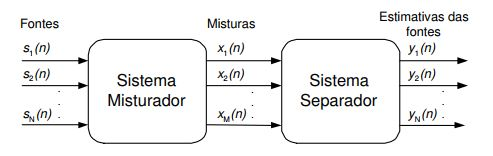
\includegraphics[scale=1.0]{fig221.JPG}\hspace*{\fill}
        \caption{Estrutura do problema de Separação Cega de Fontes.}
        \label{fig:structure}
    \end{figure}


\section{Aplicabilidade}
    Devido à generalidade do problema de BSS, várias aplicações podem ser atribuídas. Veremos, nesta seção, algumas aplicações de destaque das técnicas de BSS nas diferentes áreas.
    
\subsection{Biomedicina}
    Na biomedicina, a busca por métodos não-invasivos que ainda se mostrem confiáveis é um desafio. o EEG (Eletroencefalograma) e o ECG (Eletrocardiograma) são dois exemplos bem comuns de técnicas que satisfazem esta necessidade. Entretanto, é relativamente difícil captar apenas os sinais desejados quando os sensores são posicionados em uma determinada região do corpo humano, principalmente devido à interferência proveniente de sinais gerados por outras atividades fisiológicas.
       
    Uma forma de resolver este problema está na repetição da realização do exame, o que pode não ser viável em certas ocasiões, além de causar fadiga nos pacientes. O emprego de técnicas de BSS oferece uma alternativa eficiente, uma vez que o processamento é dado após a coleta dos dados e requer apenas um experimento.
    
    Existe uma expressiva gama de trabalhos acerca de separação de sinais biomédicos, o que evidencia sua importância.
    
\subsection{Telecomunicações}

    A BSS está diretamente ligada com um tema relevante em telecomunicações: a equalização de canais A idéia essencial de um sistema de comunicação é fazer com que a informaçãõ enviada por um transmissor possa ser obtida de maneira tão fiel ao original quanto possível por um receptor. Assim sendo, mitigar distorções introduzidas pelo canal é fundamental. Em outra estratégia, a equalização do canal, utiliza-se um filtro (equalizador) no receptor demodo que este seja capaz de anular os efeitos do canal. Em essência, o desenvolvimento de técnicas de equalização está intimamente relacionado à concepção de critérios que guiem o ajuste dos parâmetros livres do equalizador de modo que se obtenha uma boa estimativa do sinal transmitido.
    Por exemplo, em um dos paradigmas mais conhecidos, adota-se como critério a minimização do erro quadrático médio     entre a saída do equalizador e o sinal desejado, no caso, o sinal transmitido (Haykin, 1996). Os critérios presentes na equalização não-supervisionada (ou cega) utilizam, além dos sinais recebidos, apenas algumas informações estatísticas dos sinais transmitidos. Uma vantagem desta estratégia em relação ao paradigma supervisionado é a possibilidade de realizar o ajuste dos parâmetros concomitantemente com a transmissão dos dados
    
\subsection{Separação de sinais de áudio}

    Imagine a seguinte situação: uma pessoa se encontra em uma sala onde existem diversos grupos de pessoas conversando concomitantemente, como, por exemplo, em uma reunião. Além disso, há ruído de fundo gerado, por exemplo, por música ambiente e ecos no recinto. Apesar de todas essas interferências, o ser humano é capaz de distinguir a voz ou o som de interesse em um determinado momento. Essa habilidade é conhecida na literatura como \textit{cocktail-party effect} (B. Arons, 1992), justamente pela analogia com o cenário descrito.

    Este caso levou ao questionamento: será possível a um sistema de processamento artificial alimentado apenas por gravações de microfones posicionados pela sala distinguir o sinal de voz de uma pessoa qualquer? Ao passo que o cérebro humano resolve com certa facilidade este problema, o desenvolvimento de sistemas automáticos para realizar tal tarefa ainda corresponde a um complexo desafio.

\section{Modelagem Matemática do Problema}
    Neste capítulo, iremos descrever como o problema de BSS pode ser resolvido. Primeiramente, é necessário buscar modelos matemáticos capazes de expressar o comportamento do sistema em função do misturador e do separador.
    
    Considere que cada elemento do vetor $\mathbf{s}$($\mathpzc{n}$) = [$\mathbf{s_1}$($\mathpzc{n}$) $\mathbf{s_2}$($\mathpzc{n}$) \dots  $\mathbf{s_N}$($\mathpzc{n}$)] corresponde a um sinal da fonte emissora. Analogamente, representamos os sinais misturados pelo vetor  $\mathbf{x}$($\mathpzc{n}$) = [$\mathbf{x_1}$($\mathpzc{n}$) $\mathbf{x_2}$($\mathpzc{n}$) \dots  $\mathbf{x_M}$($\mathpzc{n}$)]. De forma generalizada, o sistema misturador pode ser representado pela expressão:

    \begin{equation}\label{eq:mixer}
        \mathbf{x}(\mathpzc{n}) = \mathcal{F}(\mathbf{s}(\mathpzc{n}), \mathbf{s}(\mathpzc{n-1}), \dots, \mathbf{s}(\mathpzc{n - L}), \mathbf{n}(\mathpzc{n}))
    \end{equation}
    
    onde o operador $\mathcal{F}$($\cdot$) descreve a ação do sistema misturador, L corresponde ao número de amostras passadas (memória) do vetor de fontes e o vetor $\mathbf{n}$($\mathpzc{n}$) corresponde ao ruído associado às fontes ou sensores do sistema.
    
    Vale ressaltar que a representação (\ref{eq:mixer}) tem caráter puramente didático, uma vez que não existem técnicas de BSS que lidem com todos estes efeitos representados e uma só vez. Em geral, as técnicas são aplicadas a casos específicos, isto é, versões simplificadas da formulaçao citada. Desta forma, torna-se necessário introduzir os conceitos de classificação de um sistema misturador, para auxiliar na adequação do problema para o caso proposto por este trabalho.
    
    \textbf{Sistemas Lineares vs. Não-Lineares} O sistema misturador é dito linear se o operador  $\mathcal{F}$($\cdot$) respeita o princípio da superposição, conforme descrito abaixo:

        % Linearidade
        \begin{equation}\label{eq:linearity}
            \mathcal{F}(\mathbf{a_1}\mathbf{s_1}(\mathpzc{n}) + \mathbf{a_2}\mathbf{s_2}(\mathpzc{n})) = \mathpzc{a_1}\mathcal{F}(\mathbf{s_1}(\mathpzc{n})) + \mathpzc{a_2}\mathcal{F}(\mathbf{s_2}(\mathpzc{n}))
        \end{equation}

    para quaisquer constantes $\mathpzc{a_1}$ e $\mathpzc{a_2}$ e vetores $\mathbf{s_1}$ e $\mathbf{s_2}$. Caso contrário, o sistema é classificado como não-linear. 
    
     \textbf{Sistemas Instântaneos e Convolutivos} Nos casos em que o sistema depende de amostras passadas, isto é, L$>$0, o sistema é dito convolutivo. No caso em que L=0, o sistema é dito instantâneo.
    
     \textbf{Sistema Sub-Determinado, Determinado e Sobre-Determinado} Quando o número de sensores é maior que o número de fontes (M$>$N), tem-se o caso sobre-determinado. Analogamente, o caso sub-determinado corresponde ao caso em que (M$<$N). O caso em que (M=N) é considerado determinado.
     
     Apesar da característica principal da BSS ser a falta de informação sobre o processo de mistura, é fundamental ao menos um certo conhecimento sobre a estrutura do sistema misturador. Assim, é possível definir um separador estruturalmente capaz de reverter a ação do processo de mistura. Geralmente, este tipo de aplicação é obtido com base na aplicação de interesse. No caso deste trabalho, o problema de separação de sinais de áudio, o processo de mistura é notadamente convolutivo devido à reverberações do ambiente.
     
     A maioria dos trabalhos acerca da BSS abordam cenários com sistemas misturadores lineares e com o mesmo número de fontes e sensores, diferenciando-se basicamente no contexto de misturas instantâneas ou convolutivas. Apesar desta última classificaçãço desempenhar um papel fundamental na abordagem do problema, o  processo de mistura pode ser igualmente descrito matematicamente da seguinte forma:
     
     % Notação Matricial
     \begin{equation}\label{eq:xn}
        \mathbf{x} = \mathbf{A}\mathbf{s}
    \end{equation}
    
    onde a matriz $\mathbf{A}$ de dimensão $\mathpzc{N x N}$ é chamada de matriz de mistura. A diferença é que, no caso linear, os elementos da matriz $\mathbf{A}$ são constantes que multiplicam com as componentes do vetor de fontes $\mathbf{s}$ para formar as misturas $\mathbf{x}$, enquanto no caso convolutivo, os elementos da matriz $\mathbf{A}$ são filtros \textit{FIR} que representam o percurso realizado pela fonte até o sensor, devido à reverberação. Assim, tem-se uma convolução de cada um desses filtros com cada elemento do vetor de fontes $\mathbf{s}$. A despeito de sua simplicidade, esta classe de modelos é válida
em uma vasta quantidade de problemas de BSS (\cite{ICA}). Além disso, é possível recuperar as fontes através da Análise de Componentes Independentes, que será visto na próxima seção.

\section{Análise de Componentes Independentes}
    Nesta seção, serão apresentados os aspectos basicos da ICA, relacionando-a a alguns métodos semelhantes. Embora a ICA seja definida para o caso linear e convolutivo, trataremos apenas do caso linear, pois é o que condiz com a abordagem que queremos realizar, a de separação das fontes no domínio da frequência.Recomendamos ao leitor interessado em um estudo aprofundado sobre os aspectos teóricos da ICA a leitura do trabalho de Comon (Comon, 1994), responsável pela formalização matemática desse assunto, e as referências (Hyvärinen, Karhunen &
Oja, 2001; Eriksson & Koivunen, 2004; Hyvärinen, 1999b).

\subsection{Definição}
    Devido à sua natureza recente, não é difícil encontrar ao menos duas definições distintas para a ICA. Entretanto, utilizaremos a definição que mais se aproxima com a aplicação que é o objetivo deste trabalho.
    
    \textbf{Definição 2.5.1 (ICA)} A ICA de um vetor aleatório $\mathbf{x}$ = [$\mathbf{x_1}$ $\mathbf{x_2}$ $\dots$  $\mathbf{x_M}]^T$ consiste em determinar o segundo modelo generativo linear (ou modelo ICA):
    
    \begin{equation}
        % Notação Matricial
        \mathbf{x} = \mathbf{A}\mathbf{s}
    \end{equation}
    
    onde os elementos de $\mathbf{s}$ = [$\mathbf{s_1}$ $\mathbf{s_2}$ \dots  $\mathbf{s_N}$]$^T$ são estatisticamente independentes entre si e $\mathbf{A}$ corresponde a uma matriz constante de dimensão M x N.
    

    Sob a hipótese de que os sinais fontes são estatisticamente independentes entre si, fica claro que os elementos de x não são mais independentes. O ponto fundamental da aplicação da ICA diz respeito exatamente a esta constatação, no sentido de que essa metodologia se propõe a separar as fontes a partir da recuperação da independência. O sistema separador, a matriz $\mathbf{W}$, é ajustado de modo que as compomentes do vetor $\mathbf{y}$ de estimativas das fontes sejam as mais independentes possíveis entre si.
    
    Entretanto, esta abordagem levanta a seguinte questão: tornar as estimativas das fontes independentes implica necessariamente na recuperação das fontes? Foi Pierre Comon (Comon, 1994) que naõ só respondeu a esta pergunta, mas também forneceu todo o respaldo matemático necessário para o desenvolvimento da ICA e, por consequência, da BSS.
    A partir do teorema de Darmois, ele mostrou que, de fato, é possível separar as fontes com base na recuperação da independência estatística, desde que as fontes e o sistema separador satisfaçam algumas condições.

\subsection{Separabilidade}

\subsection{Modelo de maximização da não-gaussianidade}
\subsection{Modelo de estimação por máxima verossimilhança}
\subsection{Relação com o problema de BSS}

